\documentclass[11pt]{article}
\usepackage[utf8]{inputenc} % Para caracteres en espa�ol
\usepackage{amsmath,amsthm,amsfonts,amssymb,amscd}
\usepackage{multirow,booktabs}
\usepackage[table]{xcolor}
\usepackage{fullpage}
\usepackage{lastpage}
\usepackage{enumitem}
\usepackage{multicol}
\usepackage{fancyhdr}
\usepackage{mathrsfs}
\usepackage{wrapfig}
\usepackage{setspace}
\usepackage{esvect}
\usepackage{calc}
\usepackage{multicol}
\usepackage{cancel}
\usepackage{graphicx}
\graphicspath{ {pictures/} }
\usepackage[retainorgcmds]{IEEEtrantools}
\usepackage[margin=3cm]{geometry}
\usepackage{amsmath}
\newlength{\tabcont}
\setlength{\parindent}{0.0in}
\setlength{\parskip}{0.05in}
\usepackage{empheq}
\usepackage{framed}
\usepackage{newtxmath}
\usepackage{euscript}
\DeclareMathAlphabet{\mathpzc}{T1}{pzc}{m}{it}
\usepackage[most]{tcolorbox}
\usepackage{xcolor}
\colorlet{shadecolor}{orange!15}
\parindent 0in
\parskip 12pt
\geometry{margin=1in, headsep=0.25in}
\theoremstyle{definition}
\newtheorem{defn}{Definition}
\newtheorem{reg}{Rule}
\newtheorem{exer}{Exercise}
\newtheorem{note}{Note}
\newcommand{\volume}{{\ooalign{\hfil$V$\hfil\cr\kern0.08em--\hfil\cr}}}
\newcommand{\parr}{\mathbin{\|}} % Parralel Symbol
\begin{document}
\setcounter{section}{2} %Section before the section you want. I want section 1 I put 0
\setcounter{page}{8} %page number you want to be the first page
\setcounter{equation}{16} %equation before the equation you want I want equation 2 I put 1
%\definecolor{babyblue}{rgb}{0.54, 0.81, 0.94}
\definecolor{babyblueeyes}{rgb}{0.63, 0.79, 0.95}
\definecolor{babyblue}{rgb}{0.69, 0.88, 0.9}

 \pagestyle{fancy}
 
\fancyhf{}
\rhead{Section 5:  Collisions}
\rfoot{Page \thepage}
\thispagestyle{empty}


\begin{center}
{\LARGE \bf Section 5:  Collisions}\\
{\large AE435}\\
Spring 2018
\end{center}

\vspace{5mm}
\section{Electron-Ion Collisions (Coulomb Collisions)}

Very different from electron-atom collisions.
 
Long-range forces are one characteristic distinguishing plasmas from neutral gases.  Since electromagnetic interactions have a much longer reach than atomic interactions, electron-ion cross-sections tend to be much larger than electron-neutral cross-sections.   As a corollary, the electron-ion collision frequency exceeds electron-neutral collision frequency, when the ionization fraction is above a few tenths of a percent.

\vspace{5mm}
\tableofcontents
\newpage
\subsection{Elastic}
The long-range "collision" process between electrons-ions is really a continuous process:
  \begin{center}
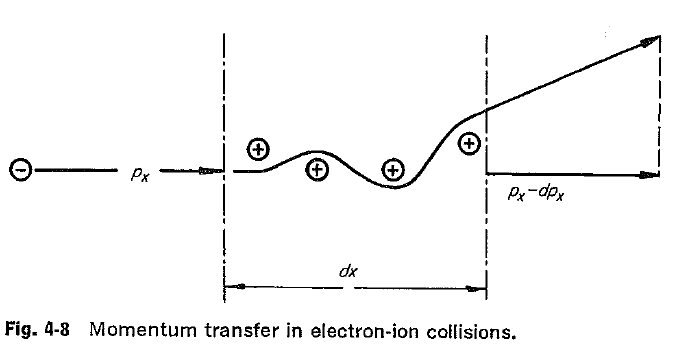
\includegraphics[scale=.9]{11.png}
\end{center}
 
Define the momentum transfer cross section                  , where x-momentum     	varies as
 
 
Then:
 
 
 
Where
           	is the relative KE before the collision
          	is an empirical cutoff distance for the effective range of the Coulomb force
 
Best choice for     	works out to be the Debye Length:
 
 
Combine logarithmic terms into the Coulomb Logarithm:
 
 
 
For a broad range of typical plasma parameters, we can simplify :
 
 
So the approximate momentum-transfer cross section is:
 
 
where Qo

\newpage
\subsection{Inelastic}
It's similar to an electron-atom collision because the electron has to penetrate into the ion core to remove another electron.

\newpage
\subsection{Radiation}
Charged particles deflected by Coulomb forces can radiate energy away as photons (bremsstrahlung).

But the energies/temperatures in EP plasmas are rarely high enough for this to be important.

\end{document}